\documentclass[12pt, letterpaper]{article}
\usepackage{amsmath}  % Enhanced math package
\usepackage{amsfonts}  % Math fonts package
\usepackage{amssymb}  % Additional math symbols
\usepackage{geometry}  % Package for setting page dimensions
\usepackage{bm}
\usepackage{textcomp}
\usepackage{graphicx}
\usepackage{caption} % for \captionof
\usepackage{listings}

\geometry{top=1in, bottom=1in, left=0.5in, right=0.5in}

\title{\textbf{\Large TPK4128 - Industrial Mechatronics Asignment 2, 2024}}
\author{Joel Perurena}
\date{January 26, 2024}

\begin{document}
\maketitle
Before going into the codes that I wrote, I want to say that I checked every link that was provided. At the end I only used 3 of the tutorial links, mainly
https://www.tutorialspoint.com/cprogramming/index.htm. I found that this tutorial had a lot of the information I was looking for. I had experience in C 
programming because I took a course in my home university, but this was almost 5 years ago. Since then I was using kind of C programming in Arduino. I 
didn't remembered many of the syntax, but while I was reading memories started to fly in. At the end I just wanted to do some programs that I could do 5 
years ago when I took the course, and implement some new things that I learned through out the tutorials.
\section*{\large Code 1}

\begin{lstlisting}
#include <stdio.h>

void compute(float x[6], int a, int b);

int main () 
{
    int a, b;
    float x[6];
    printf("Enter values for a and b to compute:\n");
    scanf("%d", &a);
    scanf("%d", &b);
    // Call to compute function
    compute(x, a, b);
    // Print the results
    printf("%d + %d = %.2f\n", a, b, x[0]);
    printf("%d - %d = %.2f\n", a, b, x[1]);
    printf("%d * %d = %.2f\n", a, b, x[2]);
    if (b != 0) {
        printf("%d / %d = %.2f\n", a, b, x[3]);
    } else {
        printf("Cannot divide by zero.\n");
    }
    printf("(%d + %d)/2 = %.2f\n", a, b, x[4]);
    printf("The greater value between %d and %d is %.2f\n", a, b, x[5]);
    return 0;
}

void compute(float x[6], int a, int b) {
    x[0] = a + b;
    x[1] = a - b;
    x[2] = a * b;
    if (b != 0) {
        x[3] = (float)a / b;
    } else {
        x[3] = 0; 
    }
    x[4] = ((float)a + b) / 2;
    x[5] = (a > b) ? a : b;

    return;
}
\end{lstlisting}
\begin{figure}[ht]
    \centering
    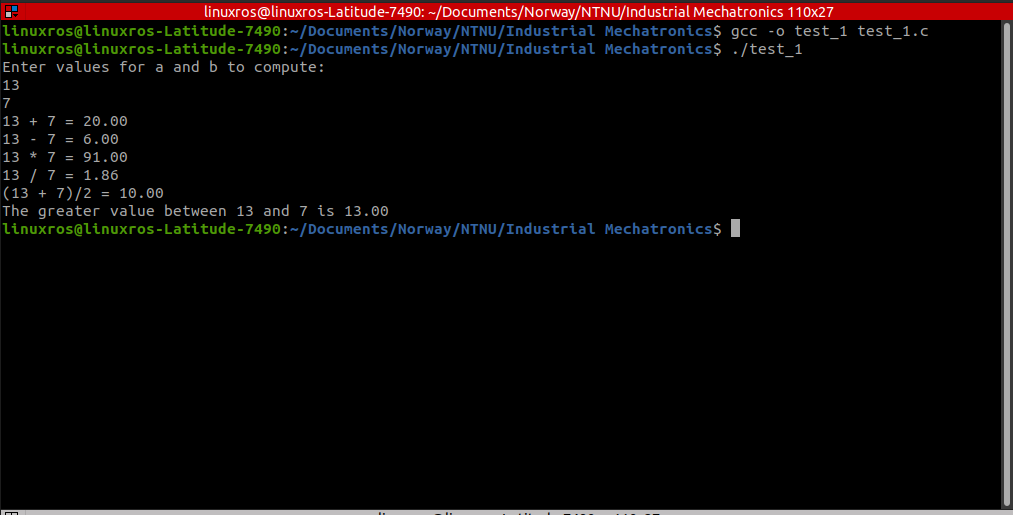
\includegraphics[width=0.8\linewidth]{test_1.png} 
    \caption{Input and Output for Code 1.}
  \end{figure}

  This code is simple but it uses a lot of C programming concepts. Mainly input and output functions like scanf and printf, void functions, arrays and
  a different way of writing an if statement by using "? :". This code is straight foward. It asks the user to input 2 interger values and those are
  saved in the variables a and b, this variables are called by the void function that computes several mathematical and logical calculations and then saves
  the values inside and x array. Then after the operations are computed, the results are printed in order by calling each element of the array.

\section*{\large Code 2}
\begin{lstlisting}
#include <stdio.h>
#include <string.h>
 
struct Student 
{
    char first_name[50];
    char last_name[50];
    char university[100];
    char faculty[100];
    int year;

};

void Student_data(struct Student student, int i);
void printStudent(struct Student student);

int main() 
{
    struct Student Student;
    int number_of_students;

    printf("How many students are going to register their data? ");
    scanf("%d", &number_of_students);

    for(int i=1;i<=number_of_students;i++)
    {
        Student_data(Student, i);
    }
    return 0;
}

void Student_data(struct Student student, int i)
{
    printf("\nStudent # %d\n",i);

    printf( "Enter your first name: ");
    scanf("%s", student.first_name);

    printf( "Enter your last name: ");
    scanf("%s", student.last_name);

    printf("Enter the name of your university: ");
    scanf(" %49[^\n]", student.university);

    printf("Enter the name of your faculty: ");
    scanf(" %49[^\n]", student.faculty);

    printf( "Enter the year you enrolled %s: ",student.university);
    scanf("%d", &student.year);

    printStudent(student);
}

void printStudent(struct Student student) 
{
    printf("\nStudent name : %s %s\n", student.first_name, student.last_name);
    printf("Univeristy : %s\n", student.university);
    printf("Faculty : %s\n", student.faculty);
    printf("Enrollment year : %d\n", student.year);
}

\end{lstlisting}
\begin{figure}[ht]
    \centering
    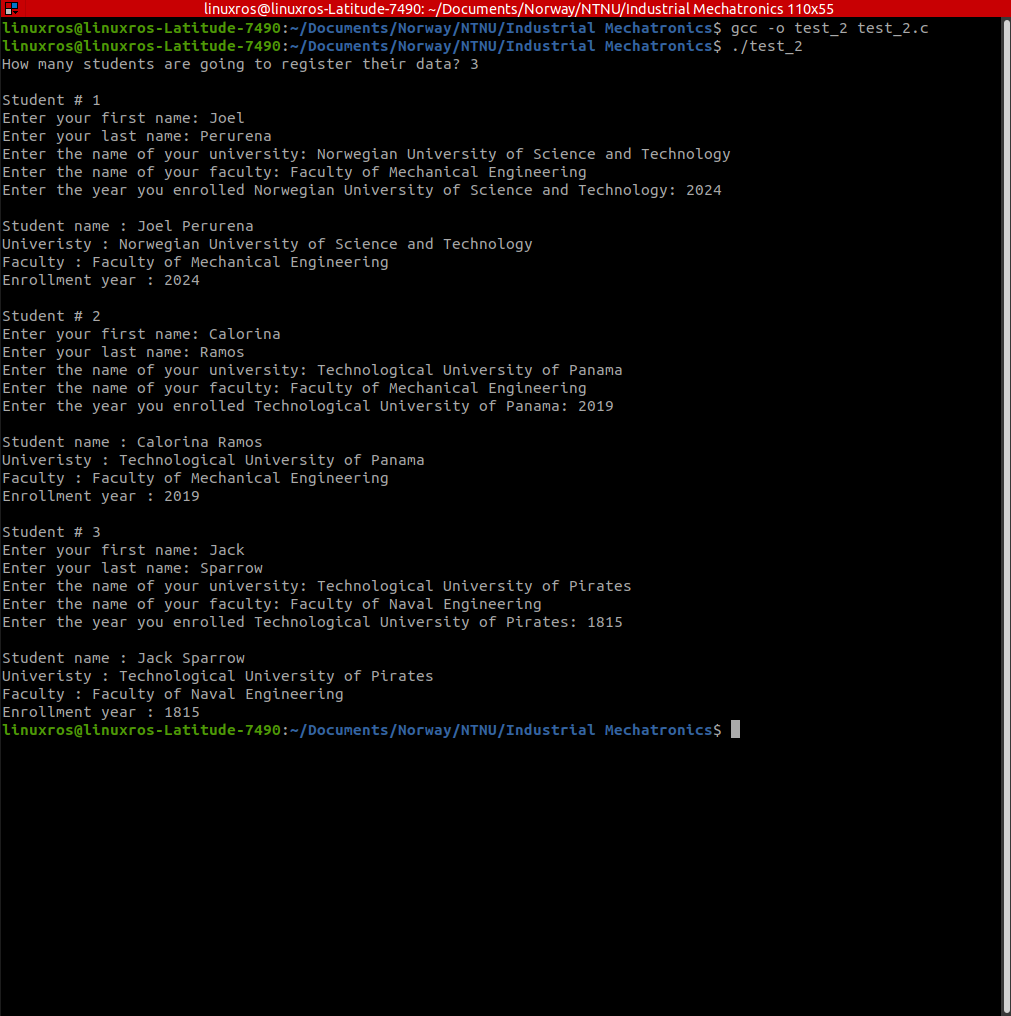
\includegraphics[width=0.8\linewidth]{test_2.png} 
    \caption{Input and Output for Code 2.}
  \end{figure}
  In this second code I wanted to explore new things that I previously didn't know. In this case it is the struct type. I wrote a program that has a struct
  type that has all the information of a student. Then in my program I ask the amount of students that are going to register their data. Using this interger value
  a for loop is called and the data is asked to the amount of students that are going to register. The registration is done inside a void function that uses
  scanf to gather the information. For the university and the faculty a different operant needs to be used because the scanf function stops when a space is
  detected, so a different operant was used to indicate the scanf function to stop reading the string just after pressing "Enter" or a new line. This way
  the student could input the whole university and faculty name without breaking the code. Inside this void function, there is another function that is called
  to print the data. This could have being done in the same function, but I wanted to try to call a function inside another function. The data is printed in
  the console.
\end{document}